{\color{indiagreen}\subsection{Definicija}}
Prefab si v Unity okolju lahko predstavljamo, kot klas GameObject-a, na katerega so pripete scipte, texture, slike, rigidbody-ji itd. To nam da možnost, da shranimo celotno GameObject-e, ki jih lahko kasneje uporabimo v sceni oz. naredimo poljubno instanc. Za boljšo pojasnitev lahko vzamemo primer drevesa. Najprej naredimo eno drevo z vsemi atributi ga shranimo in nato lahko instance v sceni in s tem dobimo efekt gozda. To lahko naredimo tudi med izvajanjem same igre, kar nam da še večje možnosti. Enako lahko naredimo za nasprotnike, zidove, zgradbe itd.
\begin{figure}[ht!]
	\centering
	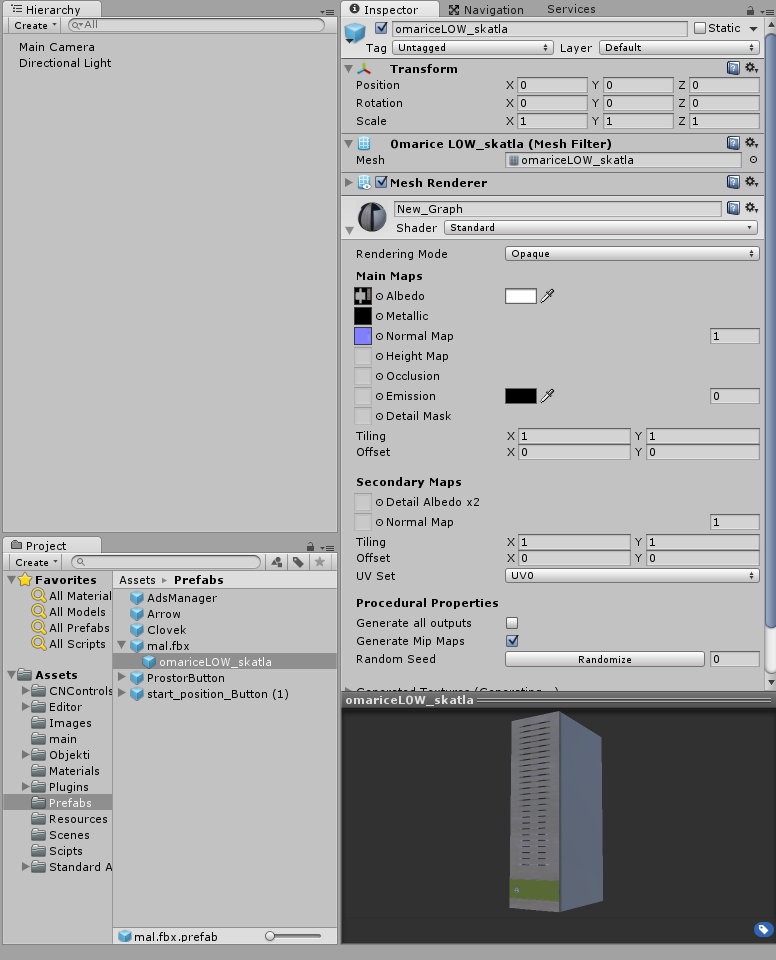
\includegraphics[width=9cm, height=12cm,keepaspectratio=true]{UnityPrefab.png}
	\caption{Prefab}
\end{figure}